\chapter{Implementácia a analýza vybraných útokov}

\label{kap:utoky}

V tejto kapitole podrobne popíšeme vybrané útoky na konkrétny hardvér, ktoré sme sa pokúsili implementovať. Zároveň sme niektoré útoky aj podrobnejšie analyzovali a následne sme sa ich pokúsili vylepšiť z hľadiska hardvéru aj softvéru. Naším cieľom bolo najmä overiť technickú náročnosť realizácie vybraných útokov a zistiť, či aj nami zvolený lacný hardvér je na takéto útoky použiteľný. Pri niektorých zapojeniach sme sa pokúsili aj presnejšie určiť (experimentálne) ako vieme ovplyvniť beh cieľového algoritmu na úrovni inštrukcií v jazyku asembler.

\section{Útok na firmvér zo súťaže CTF}
Ako prvé sme sa pokúsili zreprodukovať popísaný útok na firmvér, ktorý bol realizovaný v rámci súťaže CTF (Capture The Flag) \cite{vccOnTheCheap}. Program po spustení periodicky posiela cez rozhranie UART správu \uv{Lock}. Po úspešnom útoku by mal poslať \uv{tajný flag}, ktorého obsah je cieľom tejto súťaže. Potrebný hardvér pre realizáciu tohto útoku je nasledovný:
\begin{itemize}
    \item Arduino UNO R3 -- použili sme precízny klon, obsahuje vyberateľný čip ATMega328P v THT púzdre
    \item Arduino Nano -- taktiež precízny klon, použité na ovládanie tranzistora ako zdroj indukovanie chýb
    \item kontaktné nepájivé pole
    \item bipolárny tranzistor NPN -- model 2N2222A v THT púzdre
    \item rezistory -- použili sme 2-krát 330 $\Omega$, potrebný odpor sa môže líšiť v závislosti od použitého tranzistora
    \item prepojovacie kábliky typu M-M
\end{itemize}
Čo sa týka softvéru je potrebný ISP programátor, ktorý dokáže nahrať firmvér na mikrokontrolér ATMega328P a kompilátor jazyka C pre architektúru AVR. Použili sme integrované vývojové prostredie (IDE) Arduino IDE, ktoré poskytuje automatizovaný spôsob kompilovania a nahrávania firmvéru, podporujúce aj náš ATMega328P. Firmvér, na ktorý chceme útočiť bol zverejnený priamo v strojovom kóde a pre nahranie takéhoto kódu sme použili open source projekt AVRDUDE, ktorý interne používa aj Arduino IDE.

\subsection{Postup útoku}
Postup kopíruje popis pôvodného útoku \cite{vccOnTheCheap}. Ako prvé potrebujeme nahrať firmvér, na ktorý budeme útočiť na mikrokontrolér ATMega328P, ktorý je súčasťou dosky Arduino UNO. Doska obsahuje prevodník z USB na UART, čo zjednodušuje celý postup. Prevodník na doske pripojíme k počítaču a nahráme firmvér zo súťaže pomocou softvéru AVRDUDE \cite{vccOnTheCheap}.

Ďalším krokom je zapojenie hardvéru. Mikrokontrolér ATMega328P vyberieme z dosky Arduino UNO, keďže doska obsahuje stabilizátor napätia, ktorý by útok znemožňoval. Následne zapojíme tranzistor, tak aby ho bolo možné spínať pomocou Arduino Nano -- emitor prepojíme so zemou na doske a bázu prepojíme s pinom, ktorý ovláda tranzistor (v našom prípade pin D2). Medzi doskami prepojíme piny zabezpečujúce sériovú komunikáciu UART smerom z UNO do Nano, aby bolo možné prečítať vypísaný \uv{flag}, pre tento účel je potrebné prepojiť aj zem medzi doskami. Vybratý čip ATMega328P v púzdre THT umiestnime na kontaktné pole a prepojíme (káblikmi) spätne s pôvodnou doskou Arduino UNO nasledovné piny: 1, 2, 3, 7, 9, 10 a 20. Tieto zabezpečujú základné potreby pre fungovanie mikrokontroléra -- napájanie (zem týmto spôsobom neprepájame), hodiny (externý oscilátor), sériová komunikácia. Piny 8 a 22 (zem), prepojíme s kolektorom tranzistora. Zapnutím tranzistora pomocou výstupného pinu D2 na Arduino Nano, potom vieme odpájať a pripájať ATMega328P so zemou. Podrobná schéma celého zapojenia sa nachádza na obrázku \ref{obr:schemeCTF}.

\begin{figure}
    \centerline{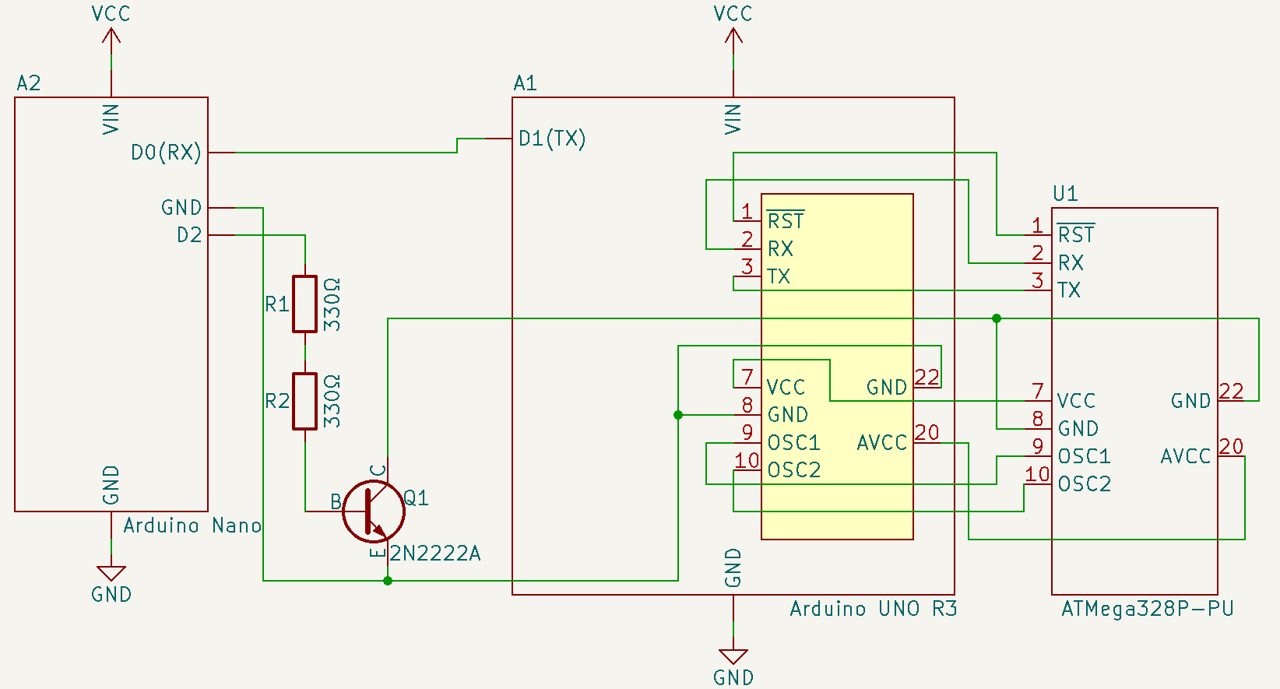
\includegraphics[width=1\textwidth]{images/schemeCTF.png}}
    \caption[Schéma zapojenia útoku na firmvér zo súťaže CTF]{Schéma zapojenia útoku na firmvér zo súťaže CTF \cite{vccOnTheCheap}. Žltý obdĺžnik znázorňuje púzdro na doske Arduino UNO, z ktorého bol vybratý mikrokontrolér ATMega328P.}
    \label{obr:schemeCTF}
\end{figure}

Ďalej je potrebné naprogramovať Arduino Nano, aby pomocou ovládania tranzistora na krátko odpojilo napájanie ATMega328P od zeme a následne opäť pripojilo. Dĺžka časového intervalu, počas ktorého je tranzistor vypnutý, musí byť dostatočne dlhá, aby indukovala chybu na procesore, ale nie príliš dlhá, aby sa mikrokontrolér reštartoval. Vyskúšali sme do Arduino Nano nahrať program použitý aj v pôvodnom útoku \cite{vccOnTheCheap}, ktorý bol implementovaný v prostredí Arduino IDE. Algoritmus vypne tranzistor a vykoná niekoľko prázdnych iterácií for-cyklu, po ktorom tranzistor opäť zapne. Následne sa pokúsi prečítať výstup zo sériového portu na ATMega328P. V prípade, že sa podarí prečítať \uv{flag}, útok bol úspešný. V prípade, že sa \uv{flag} nepodarí prečítať, zväčší počet iterácií for-cyklu a postup zopakuje \cite{vccOnTheCheap}. Ukážka časti kódu, ktorá ovláda tranzistor, je v algoritme \ref{alg:vccOnTheCheap}.

\begin{lstlisting}[float,language=C,caption={Ovládanie tranzistora, ktorý spína napájanie na ATMega328P. Prevzaté zo zdrojového kódu pôvodného útoku \cite{vccOnTheCheap}.},label=alg:vccOnTheCheap]
int waste = 0;
digitalWrite(powerPin, LOW);
for (int i = 0; i<glitchDelay; i++){ waste++; }                    
digitalWrite(powerPin, HIGH);
glitchDelay += 10;
\end{lstlisting}

\subsection{Výsledok, analýza a vylepšenie útoku}
Útok bol vyskúšaný na štyri čipy ATMega328P. Na dvoch z nich (z rovnakej série výroby) sa útok úspešne podaril s podobným výsledkom ako v pôvodnom útoku \cite{vccOnTheCheap}. \uv{Flag} sa dokonca podarilo prečítať už pri nulovom počte iterácií for-cyklu, postačoval najkratší možný výpadok -- vypnutie a okamžité zapnutie tranzistora pomocou funkcie \uv{digitalWrite} z knižnice prostredia Arduino IDE. Na druhých dvoch exemplároch (z inej série výroby) útok nebol úspešný a aj pri tomto najkratšom možnom výpadku sa mikrokontrolér reštartoval. Rozhodli sme sa preto napätie na mikrokontroléri počas útoku podrobne analyzovať pomocou osciloskopu MDO4104C, ktorý sme stručne uviedli v kapitole \ref{kap:hardver}. Pre tento účel sme sa rozhodli ATMega328P zapojiť na kontaktom nepájivom poli bez dosky Arduino UNO. Schému a detaily tohto zapojenia sme popísali v kapitole \ref{kap:hardver} a na obrázku \ref{obr:schemeATMega}. Takéto zapojenie umožňuje jednoducho meniť zapojené elektronické súčiastky, čo poskytuje väčšiu flexibilitu vo voľbe parametrov týchto súčiastok pri analýze.

Pomocou osciloskopu sa podarilo určiť priebeh zmeny napätia na mikrokontroléri v čase s presnosťou na rádovo stovky nanosekúnd. Výsledkom bolo, že interval, počas ktorého nastalo podpätie bol príliš dlhý (približne 2 {\textmu}s), čo pri útoku na 2 čipy zo štyroch spôsobilo reštart mikrokontroléra. Ďalším zaujímavým pozorovaním bol fakt, že časový interval podpätia sa nepredlžoval so zväčšovaním počtu iterácií \uv{prázdneho} for-cyklu. Dôvodom môže byť optimalizácia kompilátora, ktorý sa oprávnene rozhodol zdanlivo \uv{zbytočný} for-cyklus odstrániť.

Doska Arduino Nano, ktorá ovládala tranzistor obsahuje tiež mikrokontrolér ATMega328P, s externým oscilátorom s frekvenciou 16 MHz. V kapitole \ref{kap:hardver} sme spomenuli ukážku nastavenia výstupnej logickej hodnoty na 1, resp. 0 pomocou jedinej inštrukcie SBI, resp. CBI. Tieto inštrukcie dokáže procesor vykonať počas dvoch taktov vďaka dvojfázovej pipeline (načítanie a vykonanie inštrukcie) \cite{atmegaData}. Pri frekvencii 16 MHz to znamená, že vypnutie a opätovné zapnutie tranzistora by teoreticky malo trvať 1/4 {\textmu}s. 

Rozhodli sme sa preto časti kódu, ktoré ovládajú tranzistor prepísať do jazyku asembler s využitím C Inline Assembly, ktorý je podporovaný aj kompilátorom prostredia Arduino IDE. Volania funkcie \uv{digitalWrite} sme teda nahradili ekvivalentnou konštrukciou pomocou inštrukcií SBI a CBI. Následne sme útok zopakovali s takto upraveným programom nahratým na Arduino Nano. Výsledkom bolo, že podpätie na mikrokontroléri trvalo približne 1/2 {\textmu}s, čo je štyrikrát menej ako predtým. Dlhší čas v porovnaní s teoretickým časom (1/4{\textmu}s), bol pravdepodobne spôsobený nenulovým reakčným časom tranzistora a vplyvom ďalších fyzikálnych faktorov. Pri takto krátkom čase už nenastal reštart žiadneho z testovaných čipov, ale útok bol opäť neúspešný. Interval bol pravdepodobne príliš krátky a na žiadnom z čipov sa neprejavila chyba. Ďalej sme preto upravili kód napísaním vlastnej procedúry oneskorenia v asembleri (opäť s využitím C Inline Assembly). Procedúra pozostáva z inicializácie registra na kladnú hodnotu (osem-bitový parameter) a cyklu. V cykle postupne dekrementujeme tento register a následne vykonáme podmienený skok na začiatok cyklu, pokiaľ výsledok dekrementovania bol nenulový. Pseudokód procedúry v jazyku asembler uvádzame v algoritme \ref{alg:asmDelay}. Takáto procedúra umožňuje parametrizovať oneskorenie s presnosťou na trojice taktov (cyklus procedúry trvá tri takty). Po tejto úprave sa útok úspešne podaril na všetkých štyroch testovaných čipov. Útok bol zopakovaný niekoľkokrát (10--20), potrebné oneskorenia pre úspešný útok na každom z exemplárov sú zhrnuté v tabuľke \ref{tab:vccOnTheCheap2}. Väčšiu presnosť by bolo možné dosiahnuť pridaním presného počtu inštrukcií NOP, medzi vypnutím a zapnutím tranzistora. Počet inštrukcií NOP, by však musel byť známy v čase kompilácie, čo by znemožnilo dynamicky upravovať dĺžku oneskorenia za behu.

\begin{lstlisting}[float,language=C,caption={Procedúra oneskorenia v asembleri. \%0 označuje vstupný parameter -- hodnota v registri.},label=alg:asmDelay]
mov r24, %0   ; 1 takt
loop:
    dec r24     ; 1 takt
    brne loop   ; 2 takty pri vykonani skoku, 1 inak
\end{lstlisting}

\begin{table}
    \caption[Výsledky vylepšeného útoku zo súťaže CTF]{Výsledky vylepšeného útoku zo súťaže CTF. Každý riadok popisuje výsledok na jednom z čipov ATMega328P, na čipy zo série 2128BQY pôvodný útok nebol úspešný. Čísla v tabuľke udávajú vstupný parameter (počet cyklov) procedúry oneskorenia z algoritmu \ref{alg:asmDelay}.}
    \label{tab:vccOnTheCheap2}
    \begin{center}
    \begin{tabular}{|c|c|c|c|}
        \hline 
        Séria čipu & Min (úspešný útok) & Max (úspešný útok) & Ideál (úspešnosť nad 90\%) \\
        \hline
        2139E4A & 6 & 12 & 9--10 \\
        \hline
        2139E4A & 4 & 11 & 10 \\
        \hline
        2128BQY & 3 & 11 & 7 \\
        \hline
        2128BQY & 4 & 12 & 8--9 \\
        \hline
    \end{tabular}
    \end{center}
\end{table}

\section{Analýza zapojenia s tranzistorom}
Rozhodli sme sa ďalej podrobnejšie analyzovať priebeh napätia na mikrokontroléri medzi vypnutím a zapnutím tranzistora v predošlom útoku. Pre tento účel sme napísali jednoduchý program, ktorý periodicky zapína a vypína tranzistor. Dĺžka časového intervalu medzi vypnutím a zapnutím tranzistora je nastaviteľná pomocou analógového vstupu z potenciometra. Dĺžku tohto intervalu budeme v tejto časti udávať v počtoch iterácií procedúry oneskorenia z algoritmu \ref{alg:asmDelay}, ďalej len počet iterácií oneskorenia. Tento program sme nahrali a spustili na Arduino Nano a zapojili sme ho spolu s mikrokontrolérom ATMega328P rovnako ako vo vylepšenej verzii útoku z predošlej časti. Na vstupný analógový pin dosky Arduino Nano sme zároveň pripojili potenciometer, aby ním bolo možné regulovať počet iterácií oneskorenia. Následne sme pomocou osciloskopu MDO4104C merali priebeh napätia na mikrokontroléri, pri rôznej dĺžke intervalu medzi vypnutím a zapnutím tranzistora.

Ako sme očakávali, na mikrokontroléri periodicky vznikalo podpätie. Napätie počas vypnutého tranzistora však neklesalo prudko, ale pomaly konvergovalo k hodnote približne 2 V. Po zapnutí tranzistora sa napätie vrátilo (za čas približne 300 -- 500 nanosekúnd) na pôvodnú úroveň 5 V. Dôsledkom takéhoto priebehu bol fakt, že pri kratších intervaloch medzi vypnutím a zapnutím tranzistora napätie nestihlo klesnúť ani pod hladinu 4 V, čo už priebeh programu na cieľovom ATMega328P neovplyvnilo.

Fakt, že napätie nekleslo na 0 V, ale pokles sa zastavil pri úrovni približne 2 V, bol spôsobený tým, že k mikrokontroléru boli pripojené aj ďalšie súčiastky (najmä LED a prevodník z USB na UART). Tieto mohli mikrokontrolér nepriamo čiastočne spojiť so zvyškom obvodu aj počas zatvorenia tranzistora. Tento predpoklad sa potvrdil tým, že po odstránení týchto súčiastok a opätovnom zmeraní priebehu pomocou osciloskopu napätie už klesalo na 0 V. (Stále však rovnako pomaly.) Ako sa však v ďalších častiach ukáže fakt, že napätie neklesne až na 0 V, nebude prekážať útokom, ktoré sa pokúsime implementovať. Neskôr dokonca ukážeme, že zmena napätia až na úroveň 0 V môže byť v niektorých prípadoch až prekážať úspešnej realizácií útoku.

Rozhodli sme sa preto ku GND pinu mikrokontroléra pripojiť zdvíhací odpor. Tento odpor, by po vypnutí tranzistora mal podvihnúť napätie medzi zemou a pinom GND, čím zmenší napätie medzi napájacími pinmi mikrokontroléra postupne až k nule (VCC aj GND sa vyrovnajú na 5 V). Vyskúšali sme rôzne hodnoty zdvíhacieho odporu, pričom sme pozorovali, že efekt zdvíhacieho rezistora sa zväčšoval so zmenšujúcou sa hodnotou jeho odporu. Čím menší bol odpor, tým väčšie podpätie sa počas krátkeho výpadku podarilo dosiahnuť. Až pri hodnote 330 $\Omega$ sme pozorovali značné zrýchlenie poklesu, čo je pomerne nízka hodnota na zdvíhací odpor. Nevýhodou je potom fakt, že pri zapnutom tranzistore rezistorom preteká pomerne veľký prúd (5 V/330 $\Omega$ = 15 mA), čo sa prejavilo citeľným zahriatím odporu počas experimentu. Na obrázku \ref{obr:vccAnalysis} je porovnaný priebeh napätia na mikrokontroléri s a bez použitia zdvíhacieho odporu zaznamenaný pomocou osciloskopu.

\begin{figure}
    \centerline{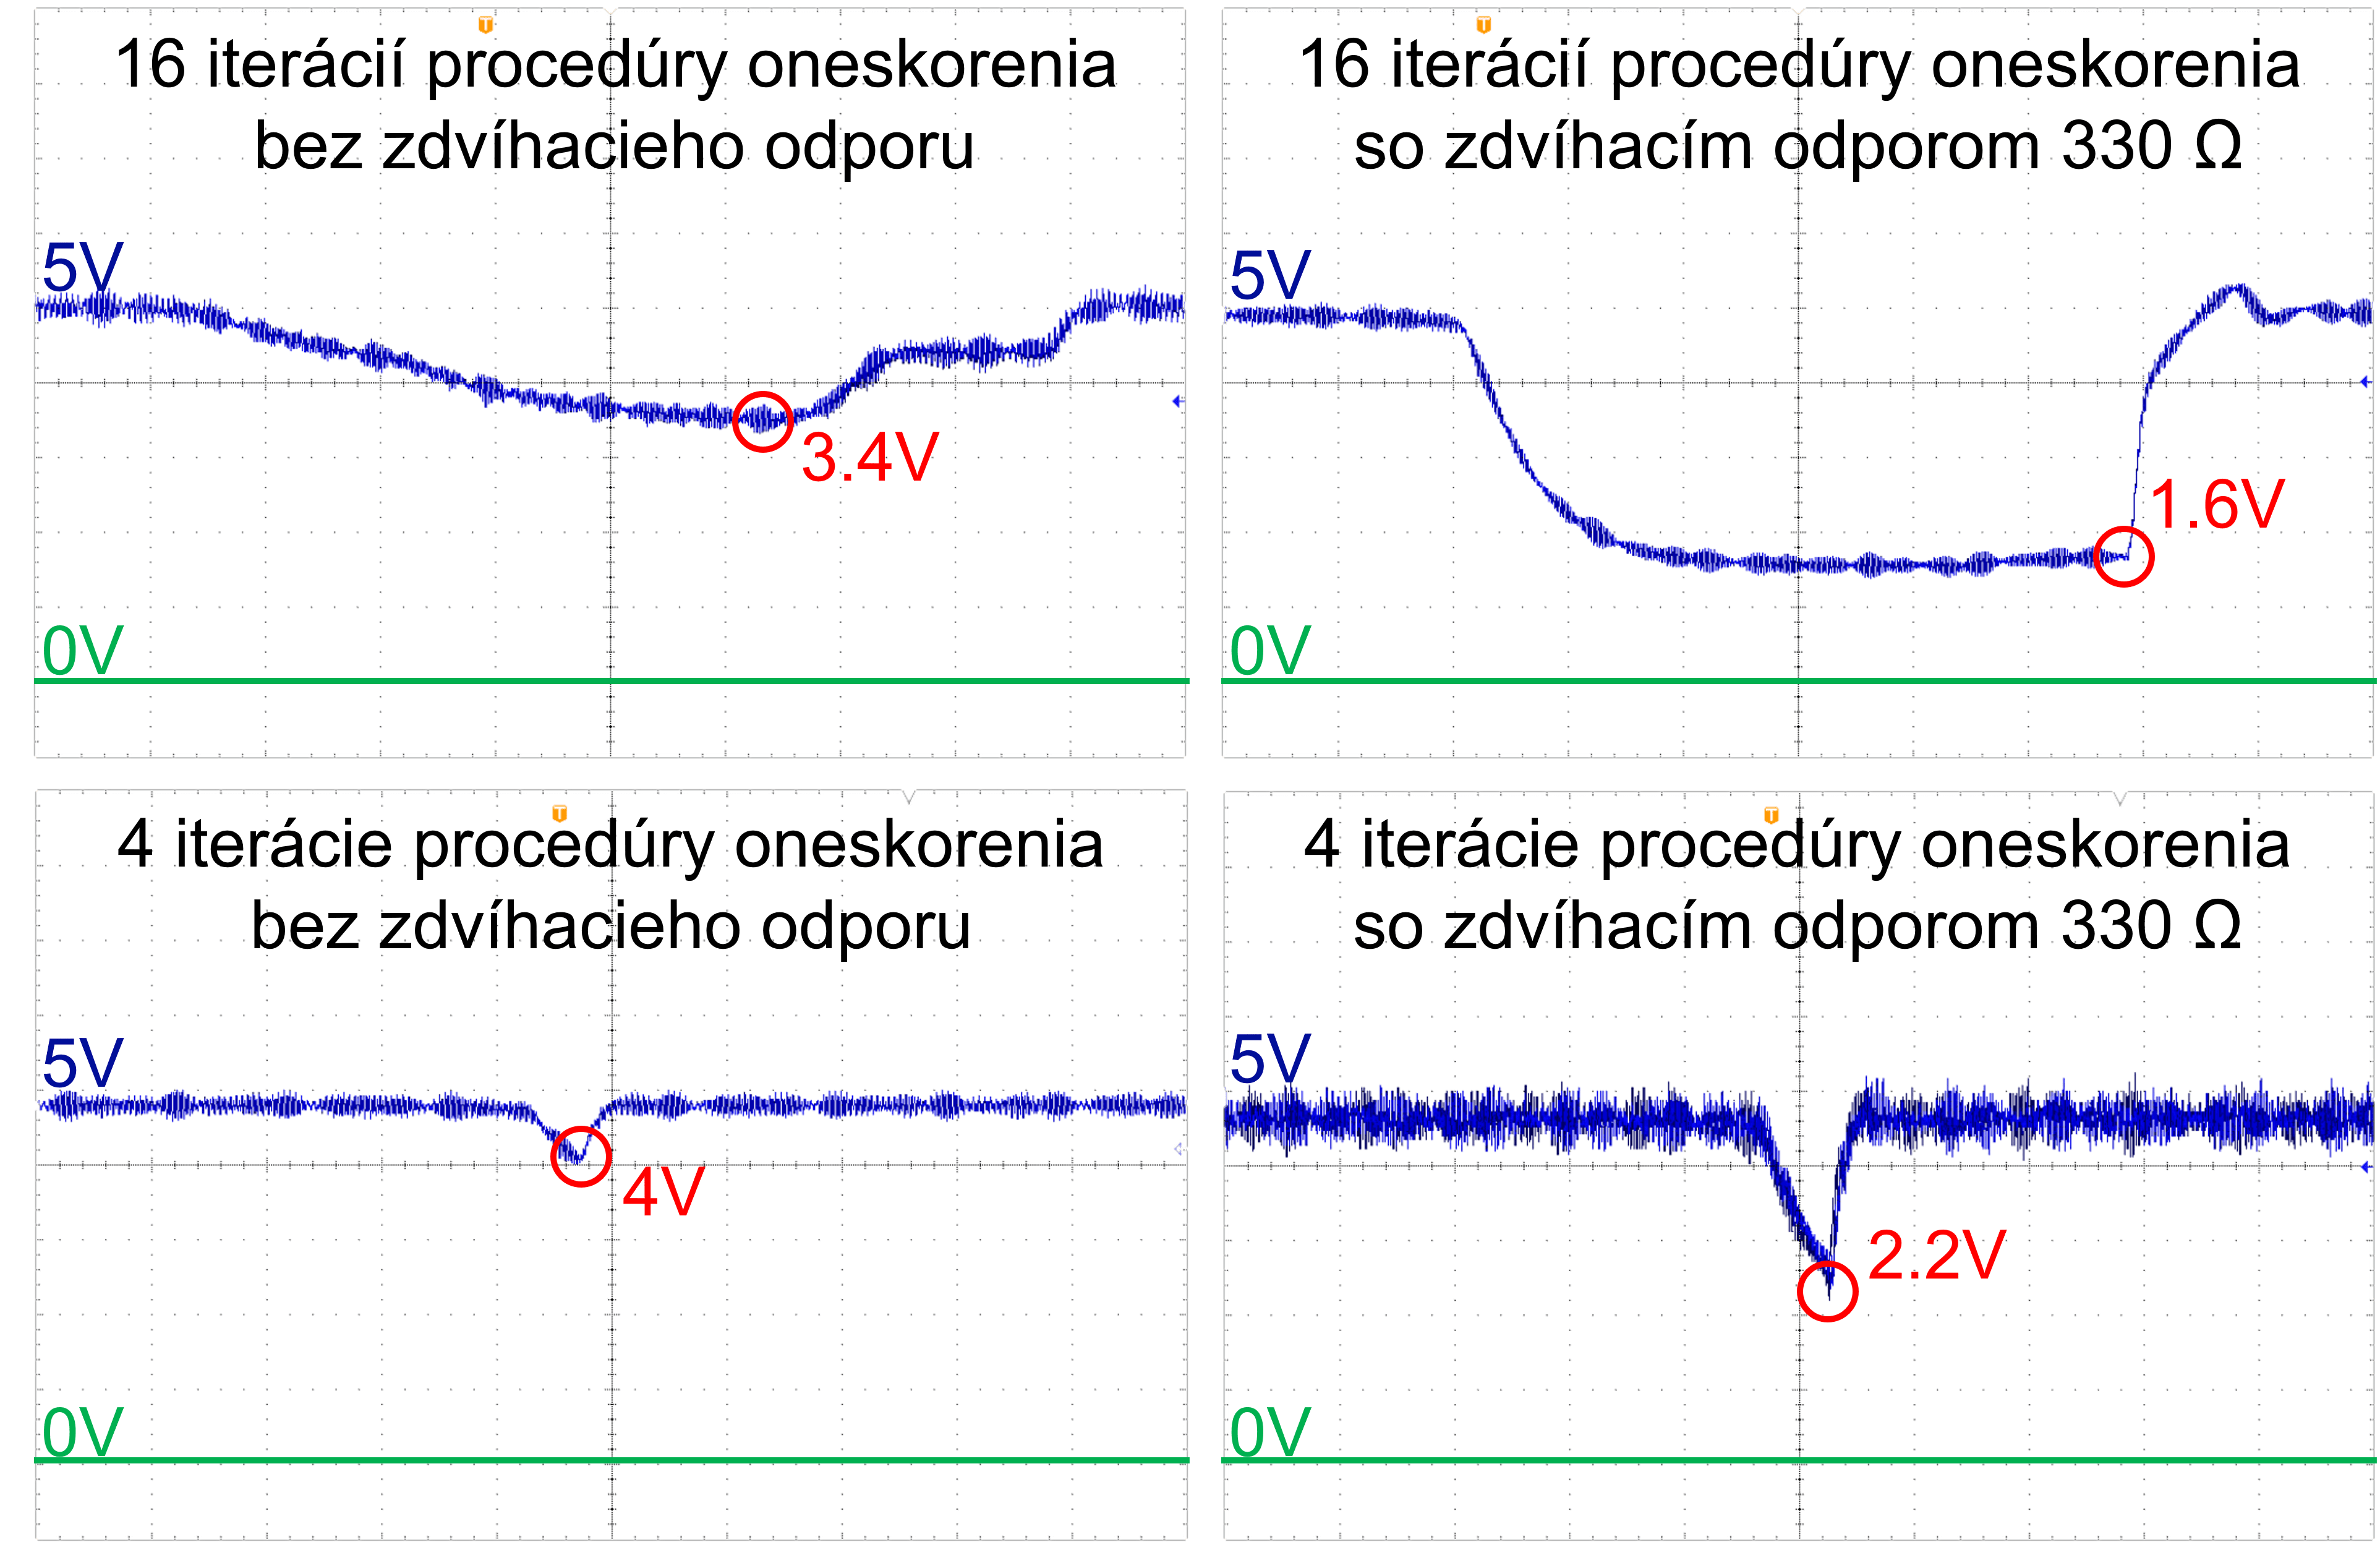
\includegraphics[width=1\textwidth]{images/vccAnalysis.png}}
    \caption[Porovnanie napätia na mikrokontroléri s/bez zdvíhacieho odporu]{Porovnanie napätia na mikrokontroléri s/bez zdvíhacieho odporu počas vypnutia tranzistora pri rôznom počte iterácií procedúry oneskorenia z algoritmu \ref{alg:asmDelay}. Veľkosť horizontálneho dielika je 400 ns. Použitý tranzistor je 2N2222A, zdvíhací odpor má hodnotu 330 $\Omega$. Modrou farbou je znázornená hodnota napätia v čase a zelená čiara v spodnej časti snímok označuje úroveň napätia 0 V. Červenou je zvýraznená minimálna nameraná hodnota napätia (zaokrúhlená na desatiny voltov).}
    \label{obr:vccAnalysis}
\end{figure}

Ďalej mohli byť príčinou takéhoto priebehu aj parametre tranzistora, ale aj niektoré pasívne súčiastky v zapojení. Rozhodli sme sa preto pozorovať ako použitie rôznych tranzistorov ovplyvňuje priebeh napätia na mikrokontroléri medzi vypnutím a zapnutím tranzistora. Vyskúšali sme tri rôzne bipolárne tranzistory -- dva typu NPN aj jeden PNP. Aby bolo možné použiť tranzistor typu PNP, bolo potrebné mierne modifikovať zapojenie. Zmena spočíva v tom, že tranzistorom budeme odpájať napájací pin, miesto zeme, čo zároveň znamená, že miesto zdvíhacieho odporu použijeme uzemňovací (s rovnakým cieľom). Okrem toho vstup do bázy, ktorý riadi tranzistor bude obrátený (logická nula zapne tranzistor). Na obrázku \ref{obr:npnVpnp} je znázornený rozdiel medzi zapojením s tranzistorom typu NPN a PNP.

\begin{figure}
    \centerline{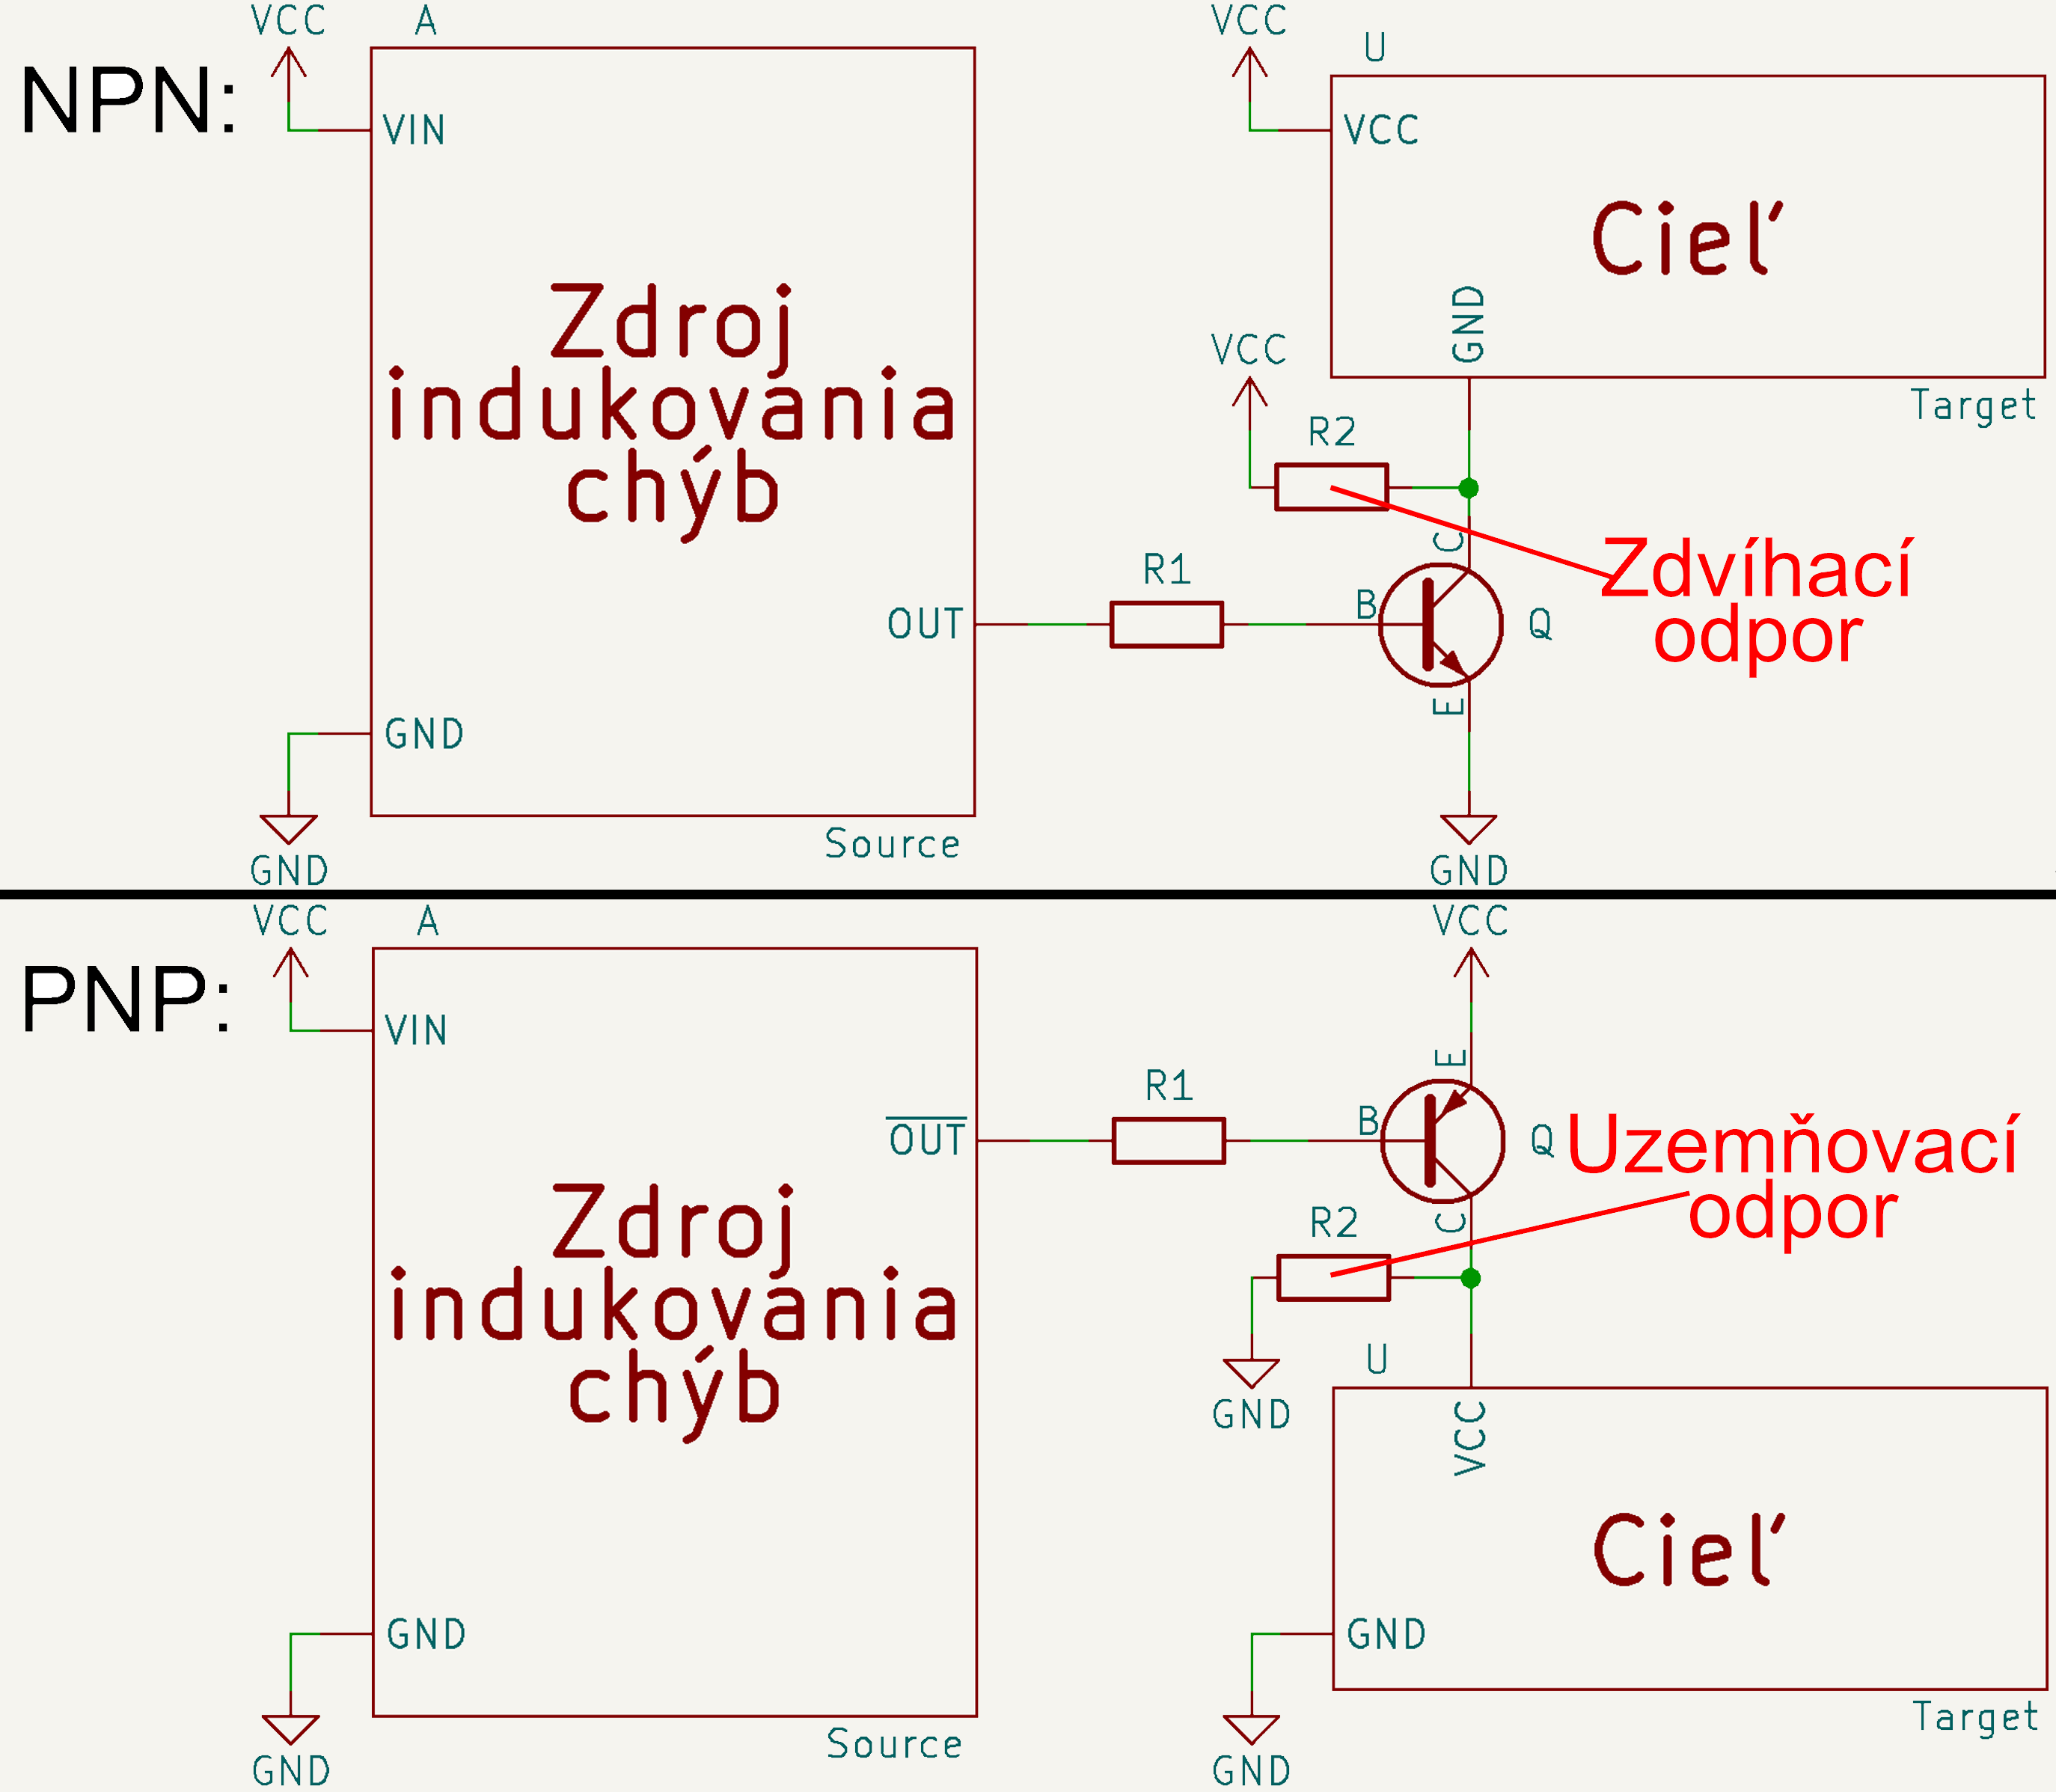
\includegraphics[width=0.8\textwidth]{images/npnVpnp.png}}
    \caption[Všeobecná schéma zapojenia s tranzistorom typu NPN a PNP]{Všeobecná schéma zapojenia s tranzistorom typu NPN a PNP.}
    \label{obr:npnVpnp}
\end{figure}

Zároveň sme každý tranzistor vyskúšali s rôznymi hodnotami zdvíhacieho, resp. uzemňovacieho odporu. Výsledky meraní sú zhrnuté v tabuľke \ref{tab:oscVoltage}, pričom \uv{víťazom}, ktorého sme sa rozhodli ponechať v zapojení pri ďalších útokoch bol tranzistor 2N2222A (NPN) so zdvíhacím odporom 330 $\Omega$ Tranzistor SS8050 mal síce kratšie časy stúpania a klesania napätia, ale minimálna úroveň napätia pri zapojení s 2N2222A bola nižšia. Dôvodom zvolenia veľmi nízkeho zdvíhacieho odporu 330 $\Omega$ bol fakt, že pri väčšom odpore bol rozdiel oproti zapojeniu bez zdvíhacieho odporu relatívne zanedbateľný. Bázový odpor tranzistora sme sa rozhodli zväčšiť na 1 k$\Omega$, keďže to neovplyvnilo priebeh napätia počas útoku a tranzistorom potečie menší prúd (stále dostatočný).

\begin{table}
    \caption[Porovnanie priebehu napätia pri zapojení s rôznymi tranzistormi]{Porovnanie priebehu napätia na mikrokontroléri pri zapojení s rôznymi tranzistormi. Hodnoty v tabuľke sú priemerom zo šesťdesiatich štyroch vzoriek -- automaticky nameraných a vypočítaných pomocou funkcie osciloskopu. Napätie je zaokrúhlené na desatiny voltov a časy sú zaokrúhlené na stovky nanosekúnd.}
    \label{tab:oscVoltage}
    \begin{center}
    \begin{tabular}{|c|c|c|c|c|c|}
        \hline
        \multicolumn{6}{|c|}{Tranzistor 2N2222A (NPN)} \\
        \hline 
        zdvíhací odpor ($\Omega$) & žiaden & 10k & 1k & 330 & 220 \\
        \hline
        min úroveň napätia (V) & 3,4 & 3,3 & 2,6 & 1,6 & 1,5 \\
        \hline
        čas od vypnutia po pokles na úroveň 3 V (ns) & N/A & N/A & 1000 & 300 & 200 \\
        \hline
        čas od vypnutia po pokles na min úroveň (ns) & 2000 & 1800 & 1400 & 1000 & 900 \\
        \hline
        čas od zapnutia po návrat na úroveň 5 V (ns) & 500 & 400 & 300 & 300 & 300 \\
        \hline
        \multicolumn{6}{|c|}{Tranzistor SS8050 (NPN)} \\
        \hline 
        zdvíhací odpor ($\Omega$) & žiaden & 10k & 1k & 330 & 220 \\
        \hline
        min úroveň napätia (V) & 2,6 & 2,5 & 2,2 & 1,8 & 1,5 \\
        \hline
        čas od vypnutia po pokles na úroveň 3 V (ns) & 1000 & 1000 & 500 & 300 & 200 \\
        \hline
        čas od vypnutia po pokles na min úroveň (ns) & 1800 & 1700 & 1000 & 900 & 900 \\
        \hline
        čas od zapnutia po návrat na úroveň 5 V (ns) & 200 & 200 & 200 & 200 & 200 \\
        \hline
        \multicolumn{6}{|c|}{Tranzistor SS8550 (PNP)} \\
        \hline 
        zdvíhací odpor ($\Omega$) & žiaden & 10k & 1k & 330 & 220 \\
        \hline
        min úroveň napätia (V) & 3 & 2,9 & 2,7 & 2,1 & 2 \\
        \hline
        čas od vypnutia po pokles na úroveň 3 V (ns) & 1000 & 1000 & 700 & 400 & 300 \\
        \hline
        čas od vypnutia po pokles na min úroveň (ns) & 1000 & 1100 & 1000 & 1200 & 1200 \\
        \hline
        čas od zapnutia po návrat na úroveň 5 V (ns) & 200 & 200 & 200 & 200 & 200 \\
        \hline
    \end{tabular}
    \end{center}
\end{table}

\section{Testovanie efektov útoku}
V tejto časti podrobnejšie preskúmame, čo presne sa dá útokom využívajúcim zapojenie analyzované v predošlej časti dosiahnuť. Pokúsime sa experimentálne určiť niektoré z možných efektov útoku na mikrokontroléri ATMega328P na úrovni makroinštrukcií procesora. Pomocou techniky zmeny napätia sa pokúsime ovplyvniť rôzne inštrukcie, prípadne kratšie časti kódu písané v jazyku asembler. Aby sme dosiahli väčšiu presnosť načasovania útoku, rozhodli sme sa pridať synchronizáciu medzi zariadením, ktoré ovláda tranzistor a mikrokontrolér, na ktorý útočíme. Tranzistor sme ovládali 2 rôznymi vývojovými doskami s rôznou frekvenciou procesora. Ako prvú sme vyskúšali dosku Arduino Nano, ďalej len Nano, s rovnakým mikrokontrolérom (ATMega328P), na aký útočíme. Ako druhé sme tranzistor ovládali pomocou dosky STM32 F4 Discovery, ďalej len Discovery, ktorá by mala mať väčšiu presnosť keďže má vyššiu taktovaciu frekvenciu -- 168 MHz oproti 16 MHz, ktorú má Nano. Obidva prístupy sme následne porovnali.

ATMega328P zapojíme tak, ako na obrázku \ref{obr:schemeATMega} na kontaktnom nepájivom poli. Zem (piny GND) zapojíme cez NPN tranzistor (aj so zdvíhacím odporom), ktorého bázu budeme ovládať pomocou výstupného GPIO pinu na zdroji indukovania chýb (Nano, resp. Discovery). Ďalej pin GPIO 8 (Port B0) na ATMega328P nastavíme ako výstupný a priamo ho pripojíme na vstupný GPIO pin zdroja indukovania chýb. Pomocou neho bude ATMega328P posielať signály pre synchronizáciu útoku. Schéma zapojenia je na obrázku \ref{obr:schemeExpTranz}. Doska Discovery neumožňuje sériovú komunikáciu s počítačom priamo cez rozhranie ST-Link, ktorým je pripojená k USB. Rozhodli sme sa preto prepojiť jej pin TX s pinom RX na ďalší samostatný prevodník z USB na UART (rovnaký model ako prevodník pripojený k ATMega328P -- obrázok \ref{obr:schemeATMega}) pre komunikáciu s počítačom na samostatnom porte.

\begin{figure}
    \centerline{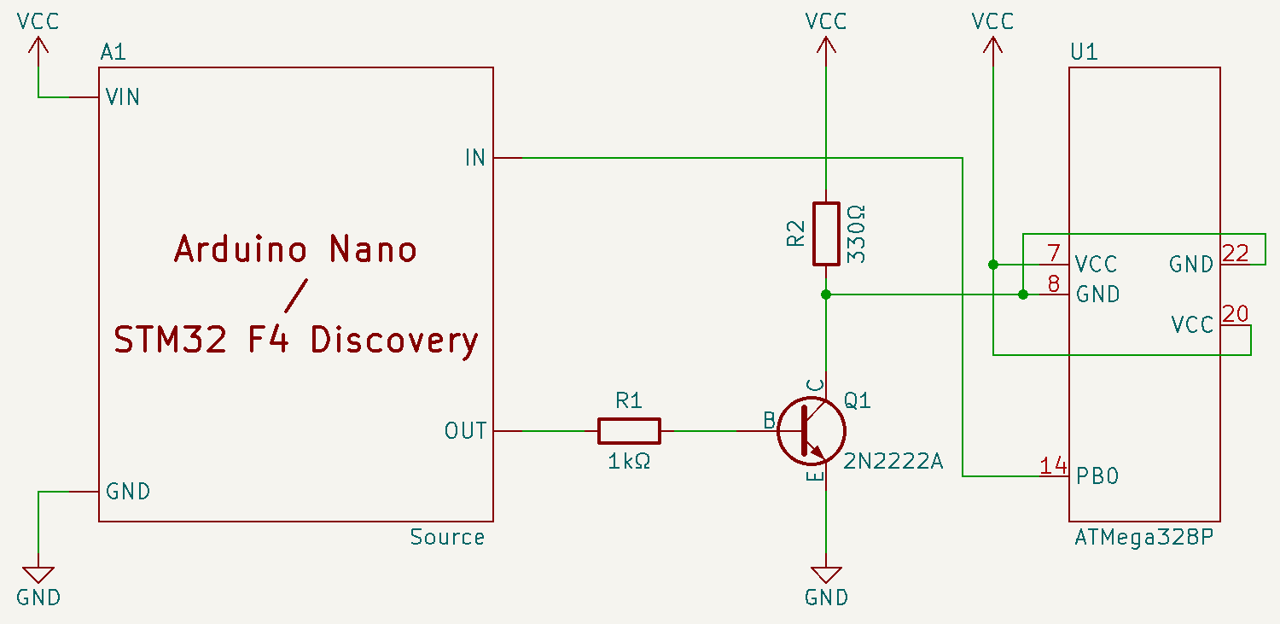
\includegraphics[width=1\textwidth]{images/schemeExpTranz.png}}
    \caption[Schéma zapojenia s tranzistorom a synchronizáciou]{Schéma zapojenia s tranzistorom a synchronizáciou medzi zdrojom a cieľom útoku. Zapojenie ostatných súčiastok k ATMega328P podľa obrázku \ref{obr:schemeATMega} nie je znázornené kvôli prehľadnosti. Prepojenie pinov PB0 a IN umožňuje posielanie signálov z ATMega328P do zdroja indukovania chýb, čo umožňuje synchronizáciu útoku.}
    \label{obr:schemeExpTranz}
\end{figure}

Experiment bude potom prebiehať nasledovne: ATMega328P pošle signál zdroju indukovania chýb a následné začne vykonávať kód, na ktorý chceme útočiť (séria inštrukcií písaná v jazyku asembler). Zdroj indukovania chýb po prijatí signálu počká krátky čas, ďalej len odstup (offset), následne zatvorí tranzistor a opäť počká krátky čas, potom tranzistor opäť otvorí. Dĺžka medzi zatvorením a otvorením tranzistora, ďalej len výpadok, a odstup sú nezávisle nastaviteľné parametre, ktorými vieme nastavovať presnosť útoku. Naše očakávanie je, že nastavením odstupu vieme zacieliť na konkrétnu časť úseku kódu, na ktorý útočíme a nastavením výpadku môžeme meniť vplyv útoku. Cieľom tejto sady experimentov bude určiť ako vieme pomocou nastavovania týchto parametrov ovplyvniť výsledok útoku. Ďalej sa pokúsime určiť aký druh chyby vieme na ATMega328P takýmto spôsobom indukovať, napríklad vynechanie inštrukcie, ovplyvnenie výsledku inštrukcie, podmieneného skoku a pod.

Pre nastavenie parametrov odstup a výpadok sme použili podobný prístup ako v algoritme \ref{alg:asmDelay}. Výhodou je možnosť nastavovania týchto parametrov aj za behu programu. Pre dosku Nano sme použili presne tú istú procedúru, zatiaľ, čo pre dosku Discovery sme navrhli analogickú, keďže architektúra jej mikrokontroléra je odlišná (podrobnosti v kapitole \ref{kap:hardver}), napríklad nepodporuje inštrukciu DEC (priamy dekrement registra). Túto inštrukciu sme nahradili pomocou inštrukcie SUBS, ktorá odčíta konštantu od registra a nastaví podmienkové bity, pre následné vykonanie podmieneného skoku. Keďže STM32F4 na doske Discovery má vyššiu taktovaciu frekvenciu, procedúra oneskorenia poskytuje väčšiu presnosť pri nastavení počtu iterácií. Porovnanie teoretickej presnosti procedúr oneskorenia sa nachádza v tabuľke \ref{tab:asmDelayT}. Z hľadiska presnosti je relevantný aj minimálny čas potrebný pre nastavenie výstupnej hodnoty na 0 a následne na 1 (napríklad na zatvorenie a okamžité otvorenie tranzistora). Túto hodnotu sme sa priamo pokúsili odmerať pomocou osciloskopu, pričom s doskou Nano sme namerali čas približne 200 ns, zatiaľ, čo pri doske Discovery len 100 ns. Tieto časy teda predstavujú dolný odhad pre časové oneskorenie riadenia akéhokoľvek obvodu. Zároveň sme sa pokúsili určiť presnosť procedúry oneskorenia. Odmerali sme dĺžku výpadku pri rôznom počte iterácií a následne sme vypočítali priemer rozdielu pri posune o 1 iteráciu. Zaokrúhlené hodnoty sú v tabuľke \ref{tab:asmDelayT}. Hodnotu parametrov odstupu a výpadku budeme ďalej v tejto časti uvádzať v počte iterácií procedúry oneskorenia pre dosku Nano resp. Discovery (napr. výpadok 5 znamená 5 iterácií procedúry oneskorenia medzi vypnutím a zapnutím tranzistora).

\begin{table}
    \caption[Porovnanie teoretickej presnosti STM32F4 a ATMega328P]{Porovnanie teoretickej presnosti procedúry oneskorenia na STM32F4 a ATMega328P. Hodnoty v tabuľke sú vypočítané na základe parametrov, ktoré uvádza príslušný výrobca \cite{atmegaData, avrInstruction, stmReference, stmInstruction}.}
    \label{tab:asmDelayT}
    \begin{center}
    \begin{tabular}{|c|c|}
        \hline
        \multicolumn{2}{|c|}{ATMega328P (Arduino Nano)} \\
        \hline 
        frekvencia procesora & 16 MHz \\
        \hline
        dĺžka 1 CPU cyklu (s využitím pipeline) & 1/16 \textmu s \\
        \hline
        počet CPU cyklov 1 iterácie (priemerný) & 3 CPU cykly = 3/16 \textmu s \\
        \hline
        nameraná dĺžka 1 iterácie (priemerná, zaokrúhlená) & 200 ns \\
        \hline
        minimálna dĺžka (inicializácia + 1 iterácia) & 3 CPU cykly = 3/16 \textmu s* \\
        \hline
        \multicolumn{2}{|c|}{STM32F4 (STM32 F4 Discovery)} \\
        \hline 
        frekvencia procesora & 168 MHz \\
        \hline
        dĺžka 1 CPU cyklu (s využitím pipeline) & 1/168 \textmu s \\
        \hline
        počet CPU cyklov 1 iterácie (priemerný) & 4 CPU cykly = 1/42 \textmu s \\
        \hline
        nameraná dĺžka 1 iterácie (priemerná, zaokrúhlená) & 20 ns \\
        \hline
        minimálna dĺžka (inicializácia + 1 iterácia) & 3 CPU cykly = 1/56 \textmu s* \\
        \hline
    \end{tabular}\\[6pt]
    *pri vykonaní iba 1 iterácie nedochádza k vykonaniu skoku a následnému sušeniu pipeline, preto dĺžka v tomto prípade môže byť kratšia ako priemerná dĺžka iterácie
    \end{center}
\end{table}

\subsection{Experimenty}
Na otestovanie efektu útoku sme napísali jednoduché úseky kódu v jazyku asembler, ktoré ATMega328P spustí hneď ako pošle signál zdroju indukovania chýb. Navrhli sme tri procedúry:
\begin{itemize}
    \item Načítanie konštanty do registra (inštrukcia LDI)\\
    Najskôr inicializujeme hodnotu registra R na 0x00 a následne doň uložíme hodnotu 0x55 (striedajúce nuly a jednotky v binárnom zápise). Cieľom útoku je ovplyvniť výsledok operácie tak, aby hodnota v registri R po vykonaní tohto kódu bola rôzna od 0x55, prípadne úplné vynechanie inštrukcie (v R ostane počiatočná hodnota 0x00).
    \item Priamy skok na adresu (inštrukcia RJMP)\\
    Inicializujeme hodnotu registra R na 0x00 a následne vykonáme skok na adresu A, ktorá sa nachádza o 1 inštrukciu ďalej. Medzi inštrukciou skoku a adresou A preskočíme inštrukciu LDI, ktorá uloží do R konštantu 0xFF). Cieľom útoku je vynechať inštrukciu skoku, čo by malo mať za výsledok, že do registra R sa uloží hodnota 0xFF (inštrukcia LDI sa nepreskočí). Za normálnych okolností by v R mala ostať hodnota 0x00.
    \item Séria inkrementov (inštrukcia INC)\\
    Opäť inicializujeme hodnotu registra R na 0x00 a následne vykonáme sériu 32 inkrementov pomocou inštrukcie INC, ktorá za každým zväčší hodnotu v registri o jeden. Pri korektnom behu by v registri R po vykonaní experimentu mala byť teda hodnota 32 (0x20). Cieľom bude pozorovať ako bude útok (s rôznymi hodnotami odstupu a výpadku) vplývať na výsledok v registri R.
\end{itemize}

Výsledkom bolo, že v prvých dvoch experimentoch bol útok neúspešný (Nano aj Discovery) -- príliš krátky výpadok nespôsobil žiadnu pozorovateľnú chybu, dlhý mal za následok úplné zlyhanie (mikrokontrolér sa síce nereštartoval, ale posielal na výstup nezmyselné správy a prestal reagovať na vstupy). Nepodarilo sa nastaviť dĺžku výpadku (binárnym vyhľadávaním) tak, aby bol výsledok útoku niekde medzi vyššie spomenutými. Zmena dĺžky odstupu výsledok neovplyvnila. Pri útoku na sériu inkrementov sa podarilo dosiahnuť, že výsledná hodnota v registri R bola 31 miesto očakávanej 32, s rovnakým výsledkom pri Nano aj Discovery.

Spomenuté pozorovanie pri útoku na sériu inkrementov naznačujú, že podpätie na mikrokontroléri počas výpadku pravdepodobne spôsobilo vynechanie jednej inštrukcie INC. Problém pri útoku v druhých dvoch experimentov mohol spočívať v tom, že kód, na ktorý cielime bol príliš krátky. Oneskorenie dané reakčným časom útočiaceho mikrokontroléra a tranzistora spôsobilo, že inštrukcia, ktorú útok ovplyvnil už nebola súčasťou cieleného kódu, ale súčasťou obsluhy rozhrania UART, ktorým ATMega328P posielalo výsledok experimentu. To mohlo mať za následok, že mikrokontrolér posielal nezmyselné správy. V horšom prípade stav pamäte nebol konzistentný z pohľadu funkcií, ktoré obsluhujú toto rozhranie, čo mohlo spôsobiť ďalšie fatálne poruchy. Pri nastavení odstupu nad hraničnú hodnotu (2 v prípade dosky Nano, 47 v prípade dosky Discovery) už nebol úspešný ani útok na sériu inštrukcií INC. Našou hypotézou teda je, že týmto útokom vieme docieliť vynechanie 1 inštrukcie, pričom musíme počítať s istým oneskorením od prijatia signálu na zaútočenie. Toto oneskorenie vieme s obmedzenou presnosťou regulovať nastavením parametra odstupu, minimálna dĺžka oneskorenia je však relatívne veľká.

Rozhodli sme sa preto modifikovať kód v ostatných dvoch experimentoch, ktoré boli predtým neúspešné. Pred inštrukciu LDI, resp. RJMP sme pridalo niekoľko inštrukcií NOP. Pridaním inštrukcií NOP by sme mali vykompenzovať oneskorenie útočiaceho mikrokontroléra, ktorý by už mal stihnúť zaútočiť na cielenú inštrukciu. Našim novým cieľom je teraz potvrdiť predošlú hypotézu a zistiť počet inštrukcií NOP, ktoré treba pridať, aby bol útok aj v prípade druhých dvoch experimentov úspešný.

Rovnaký útok sme teraz vykonali na takto modifikovaný kód (pomocou Nano aj Discovery), pričom útok sme spustili s nulovým odstupom (Hneď po prijatí signálu). Úspešne sa podarilo dosiahnuť vynechanie cielenej inštrukcie, po pridaní vhodného počtu inštrukcií NOP pred ňu. Počet bol pritom rôzny pri útočení pomocou dosky Nano a Discovery, podrobnosti sú v tabuľke \ref{tab:experiments}. V prípade inštrukcie LDI zostala v registri pôvodná hodnota 0x00 a v prípade RJMP bol register prepísaný na hodnotu 0xFF inštrukciou, ktorú mal skok preskočiť. Ďalej sme skúsili útok zopakovať aj s inými hodnotami pri inicializácií a prepísaní registra. Výsledok bol analogický, čím sme  sme potvrdili, že skutočne dochádza k vynechaniu inštrukcie a nie k inému ovplyvneniu programu. Pri určitej dĺžke výpadku a počte inštrukcií NOP bolo dokonca možné útok úspešne iterovať veľakrát za sebou so stabilným výsledkom.

\begin{table}
    \caption[Porovnanie Výsledkov experimentov]{Porovnanie Výsledkov experimentov s doskami Nano a Discovery. Veľkosť parametra výpadok je uvedený počtom iterácií príslušnej procedúry oneskorenia. Parameter odstup bol pri týchto útokoch vždy nulový.}
    \label{tab:experiments}
    \begin{center}
    \begin{tabular}{|c|c|c|}
        \hline
        zistený parameter & Nano & Discovery \\
        \hline
        min dĺžka výpadku (úspešný útok) & 4 & 50 \\
        \hline
        max dĺžka výpadku (úspešný útok) & 7 & 71 \\
        \hline
        ideálna dĺžka výpadku (najväčšia úspešnosť) & 6 & 58 \\
        \hline
        min počet inštrukcií NOP (úspešný útok) & 26 & 17 \\
        \hline
        ideálny počet inštrukcií NOP (najväčšia úspešnosť) & 27 & 19 \\
        \hline
        max počet inštrukcií NOP (úspešný útok) & 27 & 20 \\
        \hline
    \end{tabular}\\[6pt]
    \end{center}
\end{table}

Ďalej sme sa pokúsili overiť, či zmena parametra odstupu vplýva na oneskorenie útoku. Útok sme zopakovali viackrát, pričom sme postupne zväčšovali odstup. So zväčšujúcim sa odstupom sa zväčšoval aj počet potrebných inštrukcií NOP, ktoré bolo treba pridať pred cielenú inštrukciu, pričom nárast bol približne lineárny. Malé odchýlky od presnej lineárnej závislosti mohli byť spôsobené tým, že zväčšenie odstupu o 1 iteráciu procedúry oneskorenia časovo nezodpovedá presne celočíselnému násobku počtu inštrukcií NOP na cieľovom ATMega328P. Zistený vzťah medzi veľkosťou odstupu a počtom NOP inštrukcií pred cielenou inštrukciou je znázornený v grafe na obrázku \ref{obr:offsetNOP} pre hodnoty odstupu 0 -- 10. Pre presnejšie určenie tejto závislosti by bolo potrebné vykonať rádovo viacej testov. Vzhľadom na to, že počet inštrukcií NOP na cieľovom ATMega328P je statický, bolo by potrebné automatizovaným spôsobom prekompilovať a za každým nanovo nahrať výsledný program na mikrokontrolér. Našim cieľom však bolo len overiť, či zmena parametra odstupu ovplyvňuje útok. Pri skutočnom útoku je program, na ktorý sa útočí zvyčajne statický z hľadiska počtu inštrukcií v kóde a cieľom útočníka by skôr bolo správne nastaviť parametre odstup a výpadok, čo naše riešenie automatizovane umožňuje aj dynamicky za behu.

\begin{figure}
    \centerline{
        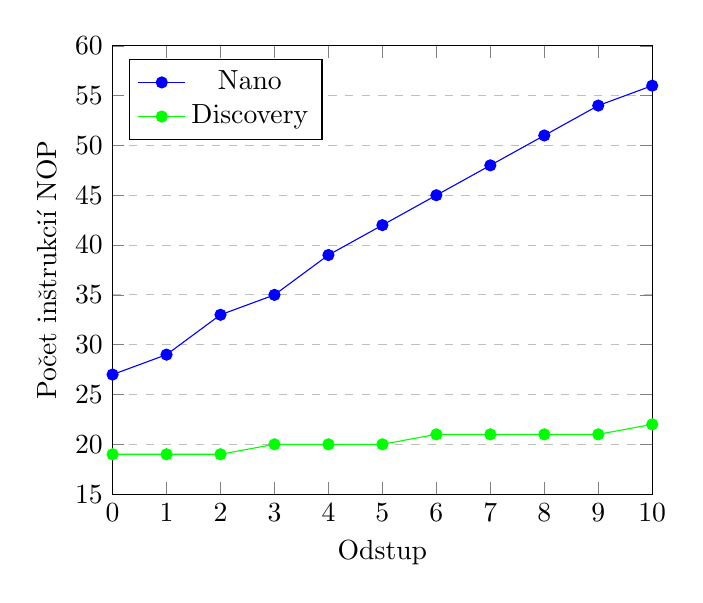
\begin{tikzpicture}
        \begin{axis}[
        xlabel={Odstup},
        ylabel={Počet inštrukcií NOP},
        xmin=0, xmax=10,
        ymin=15, ymax=60,
        xtick={0,1,2,3,4,5,6,7,8,9,10},
        ytick={15,20,25,30,35,40,45,50,55,60},
        legend pos=north west,
        ymajorgrids=true,
        grid style=dashed,
        ]
        \addplot[
            color=blue,
            mark=*,
            ]
            coordinates {
            (0,27)(1,29)(2,33)(3,35)(4,39)(5,42)(6,45)(7,48)(8,51)(9,54)(10,56)
            };
            \addlegendentry{Nano}
        \addplot[
            color=green,
            mark=*,
            ]
            coordinates {
            (0,19)(1,19)(2,19)(3,20)(4,20)(5,20)(6,21)(7,21)(8,21)(9,21)(10,22)
            };
            \addlegendentry{Discovery}
        \end{axis}
        \end{tikzpicture}
    }
    \caption[Závislosť oneskorenia útoku od parametra odstup]{Závislosť oneskorenia útoku od parametra odstup. Na zvislej osi je počet NOP inštrukcií (určený na základe úspešnosti útoku) pred cielenou inštrukciou. Na vodorovnej osi je veľkosť parametra odstup (počet iterácií príslušnej procedúry oneskorenia). Priemerný počet NOP inštrukcií na zmenu odstupu o 1 je približne 3 pre dosku Nano, resp. 1/3 pre dosku Discovery.}
    \label{obr:offsetNOP}
\end{figure}

\subsection{Ďalšie pozorovania}
Podarilo sa nám zistiť, že zapojenie s tranzistorom umožňuje cielene vynechať inštrukciu s pomerne spoľahlivou úspešnosťou. Po vhodnom nastavení parametrov odstupu a výpadku (v závislosti od cieleného kódu) bolo možné útok opakovať niekoľko krát za sebou (bez potreby reštartu cieľa) s úspešnosť nad 90\%. V niektorých prípadoch sa pri útoku na inštrukciu LDI dokonca podarilo dosiahnuť, že hodnota v registri nebola zhodná ani s pôvodnou, ani s hodnotou, ktorú mala cielená inštrukcia do registra prepísať. Pravdepodobne sa podarilo útok načasovať tak, že inštrukcia sa síce vykonala, ale s chybným výsledkom. Takýto výsledok sa však nepodarilo spoľahlivo a stabilne reprodukovať, tak aby bolo možné cielene ovplyvniť výsledok inštrukcie. Môžeme teda konštatovať, že útok vyžadujúci takéto chybné správanie by pri použitom zapojení vyžadoval použitie hardvéru s vyššou presnosťou časovania. Rovnako sa nepreukázalo, že by sa podarilo cielene ovplyvniť inštrukciu skoku tak, aby program skočil na útočníkom zvolenú adresu. Nesprávne vyhodnotenie podmienky skoku, však možno simulovať vynechaním tejto inštrukcie v prípade, že potrebujeme, aby sa skok nevykonal.

\section{Útok s využitím hradlového ovládača}
Ďalej sa pokúsime o útok pomocou hradlového ovládača, integrovaného obvodu TC4420, ktorý se stručne opísali v kapitole \ref{kap:hardver}. Pri útoku pomocou zapojenia s tranzistorom sme pozorovali pomalý pokles napätia, ktorý sme museli vykompenzovať pridaním zdvíhacieho odporu. Výrobca hradlového ovládača TC4420 uvádza, že časy stúpajúcich a klesajúcich hrán sú 25 ns \cite{gateDriver}, čo je dokonca rýchlejšie ako zapojenie s tranzistorom spolu so zdvíhacím odporom analyzované v predošlej časti.

Keďže integrovaný obvod TC4420 už obsahuje všetky potrebné súčiastky, k jeho pripojeniu k cieľovému ATMega328P nám stačia len prepojovacie kábliky a kontaktné nepájivé pole. Schéma zapojenia mikrokontroléra s hradlovým ovládačom je znázornená na obrázku \ref{obr:schemeGateDriver}. Pripomíname, že k mikrokontroléru ATMega328P sme pripojili aj súčiastky potrebné pre jeho fungovanie podľa schémy na obrázku \ref{obr:schemeATMega}. Zároveň sme ponechali prepojenie pinov z predošlého útoku, ktoré umožnilo synchronizáciu zdroja indukovania chýb z cieľom.

\begin{figure}
    \centerline{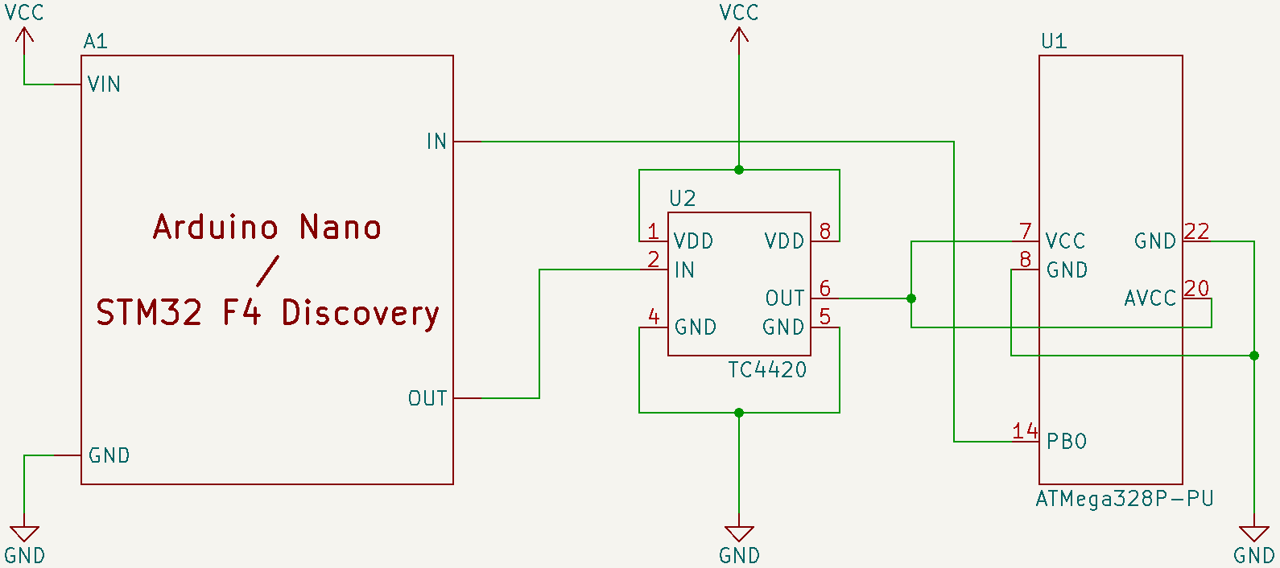
\includegraphics[width=1\textwidth]{images/schemeGateDriver.png}}
    \caption[Schéma zapojenia s hradlovým ovládačom TC4420]{Schéma zapojenia s hradlovým ovládačom TC4420. Okrem opísanej schémy sú k ATMega328P pripojené pomocné súčiastky podľa zapojenia z obrázku \ref{obr:schemeATMega}. Tie nie sú znázornené kvôli prehľadnosti.}
    \label{obr:schemeGateDriver}
\end{figure}

Následne sme sa pokúsili útokom ovplyvniť krátky úsek kódu písaný v asembleri -- séria inkrementov, analogicky ako v predošlej časti. Cieľ útoku, mikrokontrolér ATMega328P je napájaný pomocou hradlového ovládača. Tesne pred vykonaním cieleného kódu poslal signál na zahájenie útoku zdroju indukovania chýb -- Doske Arduino Nano resp. STM32 F4 Discovery. Ten následne vypol a v zápätí zapol napájanie na cieli pomocou hradlového ovládača s nastaviteľným parametrom výpadok, tak ako v predchádzajúcej časti. Výsledkom bolo, že mikrokontrolér ATMega328P sa vo väčšine prípadoch reštartoval, pri použití dosky Nano ako zdroj indukovania chýb aj v najkratšom možnom výpadku -- bez procedúry oneskorenia medzi vypnutím a zapnutím. V prípade dosky Discovery sa s nízkou úspešnosťou (približne 10\%) útok podaril a jedna inštrukcia INC bola preskočená, podobne ako pri zapojení s tranzistorom, ale len pri jednej iterácií procedúry oneskorenia. Oneskorenie dĺžky dve iterácie už spôsobilo reštart aj v prípade dosky Discovery.

Rozhodli sme sa preto opäť analyzovať priebeh napätia na cieľovom mikrokontroléri pomocou osciloskopu MDO4104C. Zistili sme, že napätie klesalo značne rýchlejšie a až na úroveň 0 V, po zapnutí sa hodnota napätia vrátila na 5 V. Pri kratších intervaloch medzi zapnutím a vypnutím napätie stihlo klesnúť po úroveň približne 1 V a zároveň pri nábehovej hrane vznikala špička s hodnotami okolo 6 V. Celý priebeh pri rôznej dĺžke medzi zapnutím a vypnutím je znázornený na obrázku \ref{obr:gateDriverAnalysis}.

\begin{figure}
    \centerline{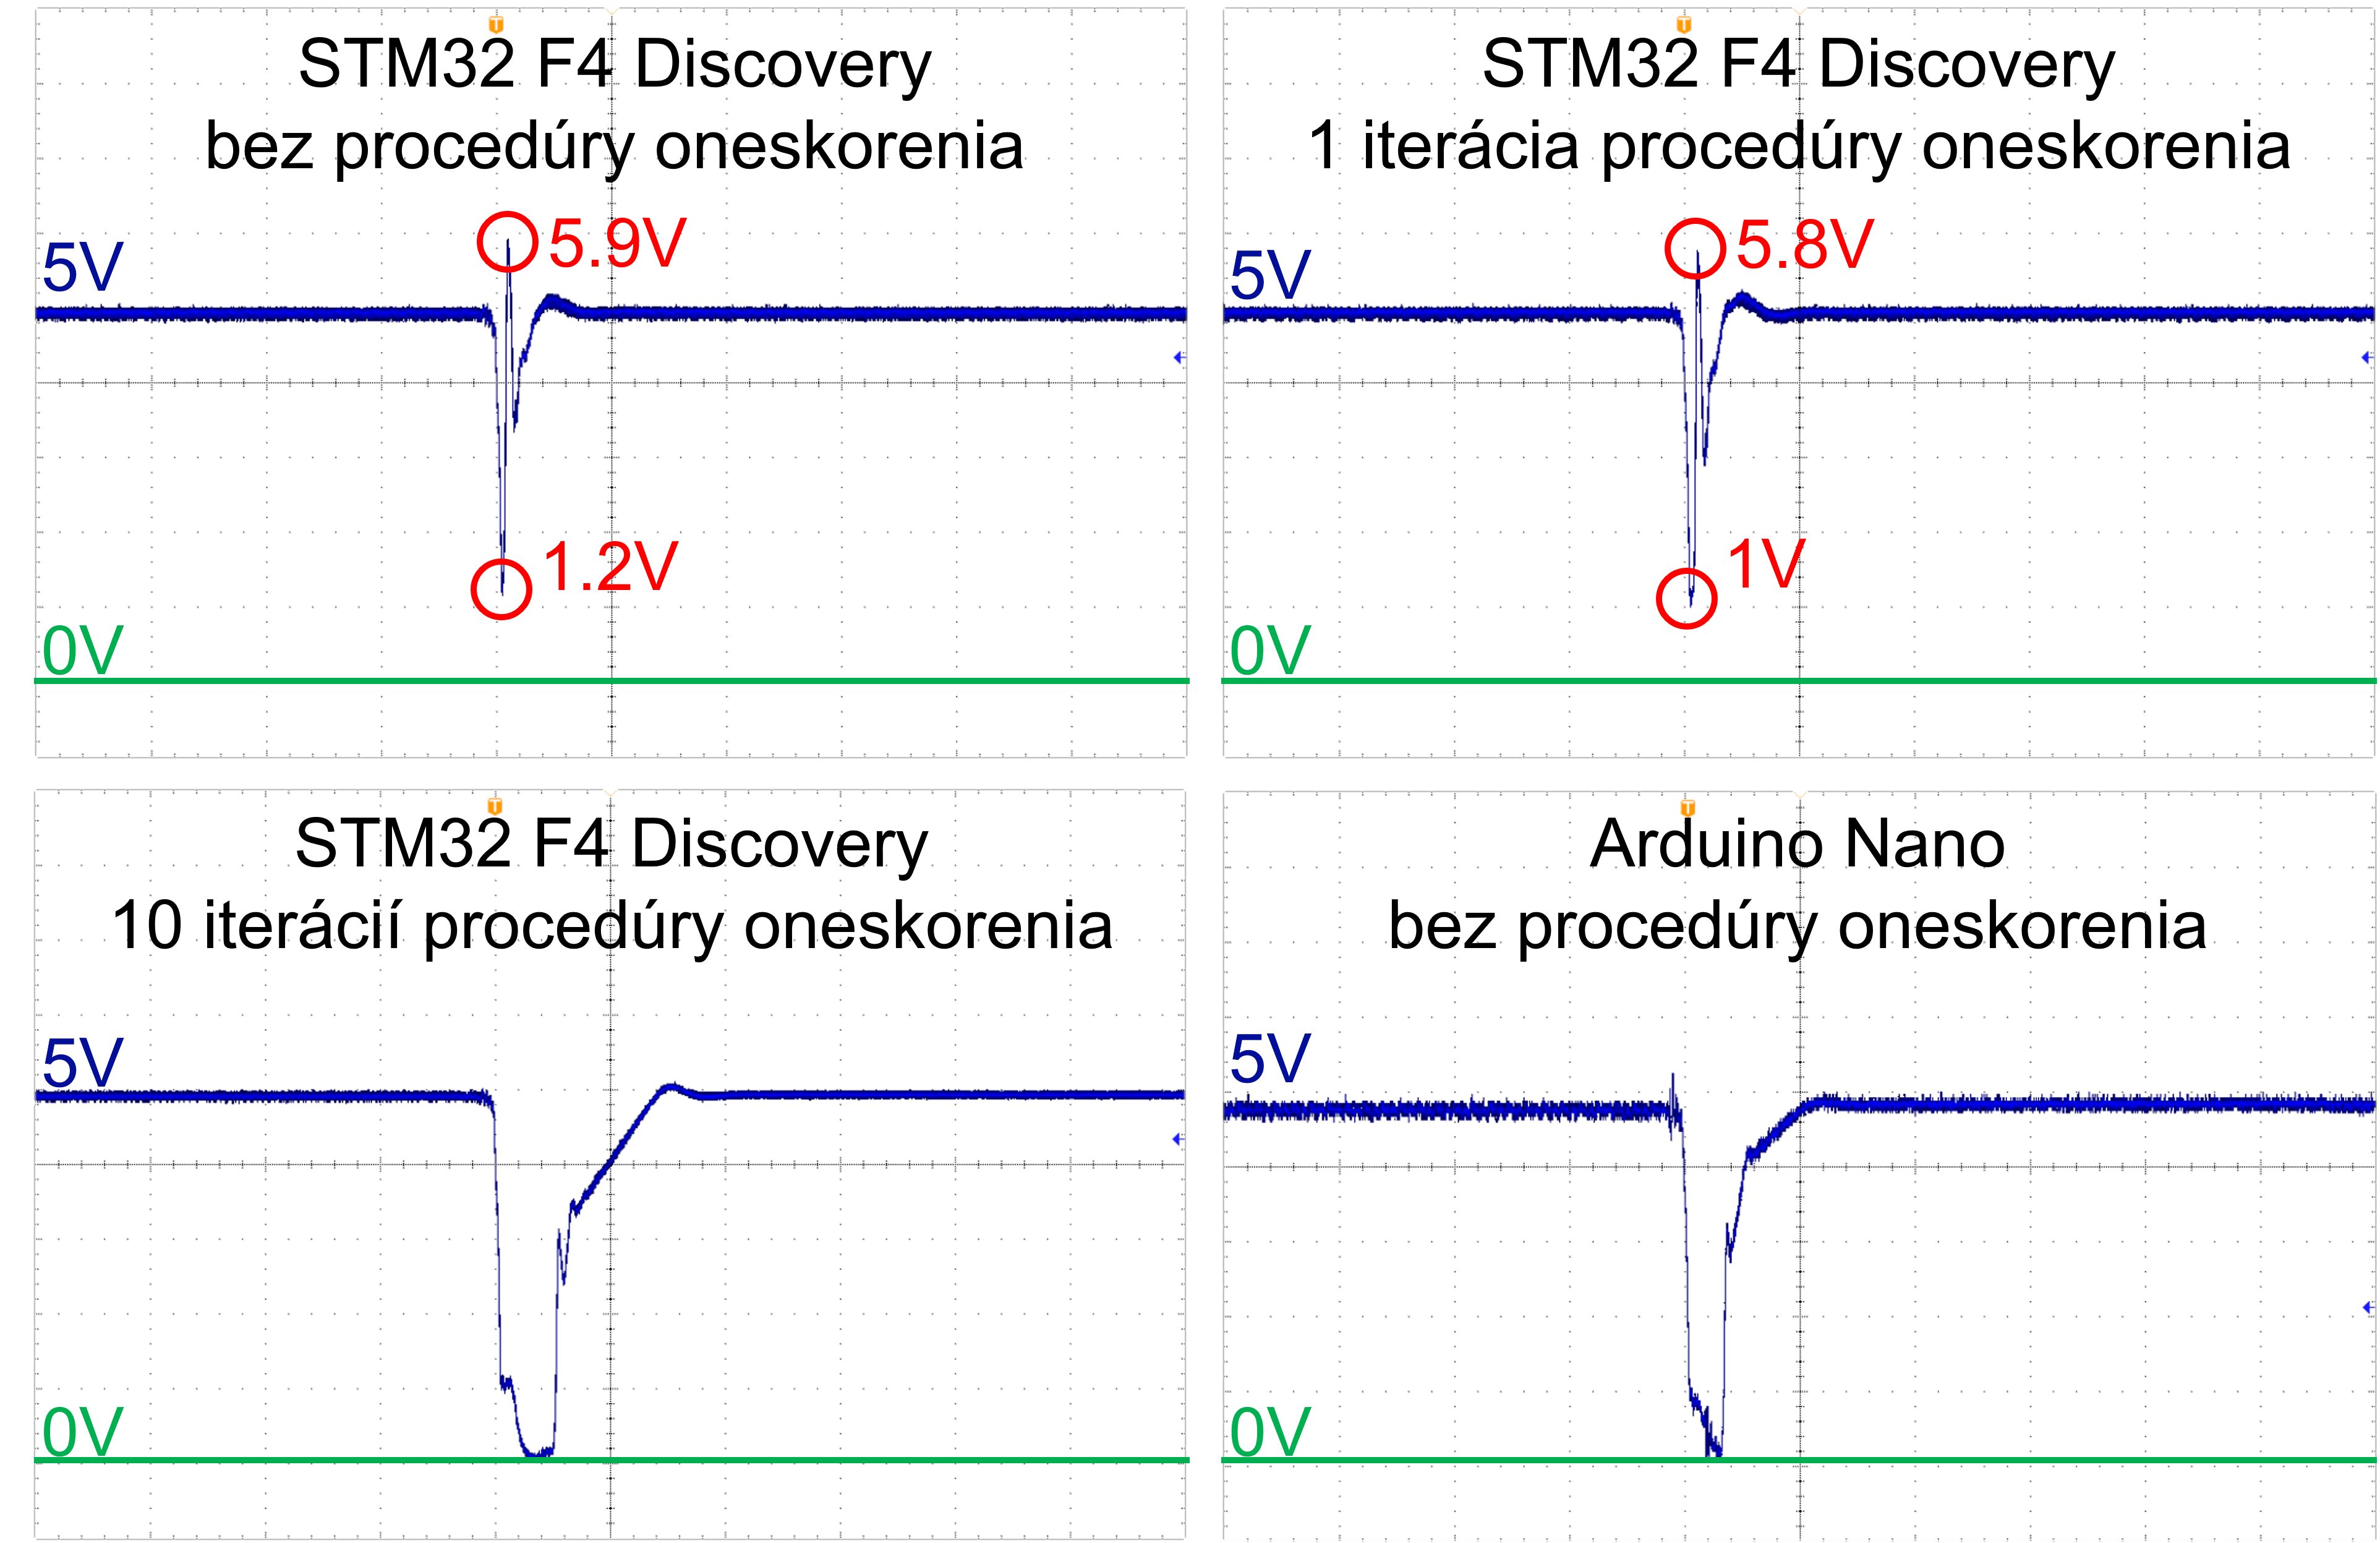
\includegraphics[width=1\textwidth]{images/gateDriverAnalysis.png}}
    \caption[Priebeh napätia na mikrokontroléri pri útoku hradlovým ovládačom]{Priebeh napätia na mikrokontroléri pri útoku pomocou hradlového ovládača. Na obrázku je znázornený priebeh pri rôznom počte iterácií procedúry oneskorenia pri ovládaní doskou Discovery. Vpravo dole je priebeh napätia pri ovládaní pomocou dosky Nano bez procedúry oneskorenia. Veľkosť horizontálneho dielika je 400 ns. Použitý hradlový ovládač je obvod TC4420. Modrou farbou je znázornená hodnota napätia v čase a zelená čiara v spodnej časti snímok označuje úroveň napätia 0 V. Červenou sú zvýraznené významné hodnoty napätia v čase (zaokrúhlené na desatiny voltov).}
    \label{obr:gateDriverAnalysis}
\end{figure}

Na základe analýzy môžeme konštatovať, že dôvodom neúspešnosti útokov pri zapojení s hradlovým ovládačom je pravdepodobne prudký pokles napätia až na 0 V a pomalá reakcia nami zvoleného hardvéru pre riadenie útoku. Interval, počas ktorého vzniklo podpätie bol príliš dlhý a preto väčšia kvalita zapojenia s hradlovým ovládačom v porovnaní s tranzistorom sa ukázala ako nežiadúca. Pri zapojení s tranzistorom fakt, že napätie klesalo počas vypnutia pomalšie, kompenzoval nízku presnosť použitého lacného hardvéru, čo v konečnom dôsledku prispelo k úspešnosti útokov. Pri použití dosky Arduino Nano sa pomocou hradlového ovládača nepodarilo realizovať ani jeden úspešný útok. Pomocou dosky STM32 F4 Discovery sa útok síce podaril, ale, ako sme spomenuli, s rádovo nižšou presnosťou ako pri zapojení s tranzistorom. Preto sme sa rozhodli týmto útok pomocou hradlového ovládača uzavrieť s tým, že k jeho úspešnému použitiu na útok pomocou techniky zmeny napätia by bol potrebný lepší hardvér s vyššou presnosťou, napr. FPGA alebo laboratórny zdroj. Napriek tomu sme analýzou potvrdili, že z hľadiska presnosti a reakčného času mal hradlový ovládač lepšie vlastnosti ako tranzistor.